\chapter{Experiments}
\label{sec:experiments}
This chapter introduces the line of experiments taken out in this work and their intermediate conclusions. Initially, basic experiments about the detection of \acp{EWFO} are conducted. In further steps the insights are applied when transferring to the more challenging environment of autonomous drone races. Finally, a detector for \acp{EWFO} is deployed on an example \ac{MAV}.

\section{Experimental Setup}

The section gives an overview of the hardware used for training as well as details on the training process. Furthermore a description of particular plots used for evaluation is given.

As training a neural network is a computationally intense process common practice is to use \acp{GPU} for faster execution. In this work all trainings are carried out on a Nvidia Pascal GTX 1080 Ti GPU with 3584 cores and 11GB RAM.

The training is stopped when the performance on unseen examples does not further improve. Therefore 0.1 \% of the training samples are used as validation set. The training is stopped when the validation error converges; that is when it does not decrease for more than $1e^{-08}$ in 3 epochs.

The detector is tested by inferring the network on a given test set and calculate the metrics described in \Cref{sec:metrics}. While this gives a good estimation about the overall performance of a network it can be required to investigate the results in greater detail. It can be important to now how the detector deals with certain view points for example. In order to perform this evaluation predictions and true labels are assigned on bins based on certain conditions e.g. the bounding box size. Subsequently the performance is evaluated only for each bin individually.

In special cases it can happen that a bin border falls right between a true and a predicted label. For example a prediction is of size 10 a predicted label of size 12 and the border is at size 11. Even if the detection is correct this separation would lead to counting a missing detection as well as a false positive in each of the bins. Hence, the performance for the individual bins is typically a bit lower than when calculating a metric for the whole dataset.

The training algorithm as well as the network initialization are random processes. Hence, the network weights after training, as well as its performance are not deterministic. This condition has to be taken into account when interpreting the results. Ideally, each training is performed repeatedly and mean and standard deviation are used for evaluation. However, the training of \acp{CNN} takes a considerable amount of time which is why not all experiments can be taken out with many repetitions. Instead, trainings are performed at least two times and only further repeated if the two results have a high deviation. In plots an error bar displays the standard deviation between the different repetitions.


\section{Evaluation Metrics}
\label{sec:background:metrics}
The detection performance is evaluated in terms of precision and recall. These metrics are defined as:

\paragraph{Precision}
$$p = \frac{\text{true positives}}{\text{true positives} + \text{false positives}}$$

\paragraph{Recall}
$$r = \frac{\text{true positives}}{\text{true positives} + \text{false negatives}}$$

Where true positives are objects that are detected, false positives are detections although there is no object and false negatives are objects which have not been detected.

Hence, recall expresses how many of all objects are detected and therefore how complete the result is. Precision measures how many of the predicted objects are actually correct detections.

A correct detection is determined based on its overlap with a ground truth box. This is measured by the relation of \ac{IoU}. In experiments we determine 0.6 as sufficient overlap for a detection. 

The model used within this thesis associates a "confidence" value with each prediction that can trade off precision and recall. This is further explained in \Cref{sec:object_detection}. By accepting more detections with a lower confidence threshold, the probability increases that one of the predictions is a true positive. Hence, it increases recall. However, it also increases the probability of false positives and thus lowers precision. In order to evaluate this trade-off precision and recall can be compared at different confidence levels.

A metric that combines precision and recall in a single metric is average precision $ap$ introduced by the Pascal Visual Object Challenge (Pascal VOC)\cite{Everingham2010}. It takes the average interpolated precision $p_{interp}$ across evenly spaced recall levels:

$$ ap = \frac{1}{11}\sum_{r \in {0,0.1,...,1.0}}p_{interp}(r)$$

The interpolation reduces the amount of zig-zags in precision-recall plots and simplifies the comparison between outputs off different detectors. It is defined as:

$$ p_\text{interp}(r) = \max\limits_{r' \geq r} p(r')$$

We denote precision, recall and average precision at a certain \ac{IoU} threshold such as 60\% as $p_{60}$,$r_{60}$ and $ap_{60}$.

\section{Threats to Validity}

\section{Empty Objects}
\label{sec:empty}
\acp{CNN} combine simple local features to more complex patterns layer by layer. Thereby pooling removes task irrelevant information and reduces the spatial dimension. In the deeper layers features of larger areas in the image are combined and encoded in an increasing amount of filters. In the final layer each location in the volume encodes the patterns that are present in the respective field of the preceding filters and an object prediction is performed.

The power of deep \acp{CNN} arises from their capability to learn very complex patterns. However, these are not present in \acp{EWFO}. Instead most of the object area consists of background and should be ignored by the detector. We hypothesize that this emptiness makes the detection more difficult than the detection of other objects as the detector can not exploit complex patterns. Instead any object can be present within the frame and thus distract the detector.

The combination of emptiness and simple features can have further implications on the training of an Object Detector for \acp{EWFO}. If not sufficient variations in background is provided in the training set, a detector is likely to overfit to the background of the training set. This condition can be amplified for more complex architectures with more parameters.

To summarize our hypotheses are:
\begin{enumerate}
	\item Compared to a simple filled object, the detection of \acp{EWFO} is harder, as the object does not provide complex patterns and a detector can be confused by patterns that are present in the empty part. 
	\item Compared to a complex filled object, the detection of \acp{EWFO} can not be improved by using a deeper network.
	\item Compared to other objects \acp{EWFO} do depend more on background. If the environment in the training set is different to the test set, the performance drop for \acp{EWFO} is higher than for other objects. 
\end{enumerate}

In order to evaluate these hypotheses the detection of an \ac{EWFO} is compared to a comparable object where the empty part is filled with a certain pattern. The created objects \textit{Cats} and \textit{Sign} are visualized in \Cref{fig:cats}. Thereby a simple object is chosen such as the stop sign which is clearly distinguishable from the background. This is compared to a more complex object such as the cat image.

The created objects allow to study how a detector performs that is trained on a filled object. Also, it allows to study how the detector for \acp{EWFO} reacts when during testing another pattern is present in the empty part.

\begin{figure}[hbtp]
	\centering
	\begin{minipage}{0.3\textwidth}
		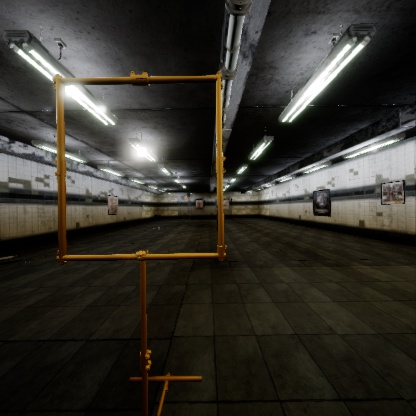
\includegraphics[width=\textwidth]{fig/gate}
	\end{minipage}
	\begin{minipage}{0.3\textwidth}
		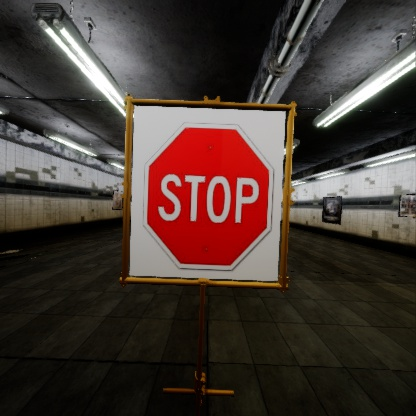
\includegraphics[width=\textwidth]{fig/sign}
	\end{minipage}
	\begin{minipage}{0.3\textwidth}
		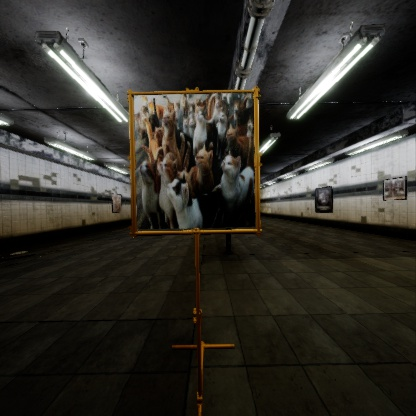
\includegraphics[width=\textwidth]{fig/cats}
	\end{minipage}
	\caption{Examples of the three objects that are compared. The \acp{EWFO} object (\textit{Gate}) left is compared to a simple solid object (\textit{Sign}) in the center and a complex solid object on the right (\textit{Cats}).}
	\label{fig:cats}
\end{figure}

For each object a dataset with 20 000 samples is created within the \textit{Dark} environment. As this experiment focuses on the influence of the empty part of the object, the view points are limited to frontally facing the object in various distances. On these training sets the two architectures illustrated in \Cref{sec:meth} \textit{SmallYoloV3} and \textit{VGGYoloV3} are trained. As 20 000 samples is a comparatively small amount of samples for a network such as the \textit{VGGYoloV3}, the network is initialized with the weights of the \textit{VGG-19} pretrained on ImageNet.

For each object a test set of 200 samples is created within the \textit{Dark}-Environment, as well as the \textit{IROS}-Environment. Hence, in total there are 6 test sets with 150 samples each. Similar to the training set the view points are limited to frontally facing the object at various distances.



\subsection{Results}

\begin{table}[hbtp]
	\centering
	\input{tables/all_basement.txt}
	\caption{Performance of two architectures when the test environment is similar to the training environment. Each trained network (row) is evaluated on each test set (column). It can be seen how the detectors exploit the structure that is placed in the object. In contrary, the detector of \acp{EWFO} only gets confused when the structure inside the object is very different from the training set.}
	\label{tab:all_basement}
\end{table}

\Cref{tab:all_basement} shows the results in the \textit{Dark}-environment. It can be seen how the best results are obtained for the \textit{Cats}-object. Yet when the structure is removed the performance drops almost to zero. A similar observation can be made for the \textit{Sign}-object. In both cases the performance can not really be improved by using a deeper network.

For detecting the \textit{Gate}-object, the lowest performance is achieved. When the same detector is applied on an object where the empty part is filled, the performance drops. This happens particularly for the \textit{Sign}-structure. For the \textit{Cat}-structure the performance drop is lower. In fact for the deep network there is not really a performance drop measurable.

\begin{table}[hbtp]
	\centering
	\input{tables/diff_iros.txt}
	\caption{Change in performance when the detectors are tested in another environment than their training environment. The most severe drop can be seen at the \textit{Cats}-object. The drop for \acp{EWFO} is comparable to the \textit{Sign}-object}
	\label{tab:diff_iros}
\end{table}

\Cref{tab:diff_iros} shows the change in performance when the trained detectors are applied in a different environment. All detectors are subject to a significant drop, however the strongest effect can be seen for the \textit{Cats}-object. While the \textit{Sign}-object can still be detected best, its relative performance drop is comparable to the \textit{Gate}-object. The network size does not have a significant effect when changing the test environment.

\subsection{Discussion}

It can be seen how the detector exploits the added structure in the filled objects. The performance is much better than for the \textit{Gate} object. Also, when the detectors trained with added structure are applied on the empty object the performance drops. Thereby the network size is of minor effect. No performance boost is achieved even for the more complex \textit{Cats} object.

When the test environment changes, the most complex object can almost not be detected anymore. It seems that the detector particularly overfitted to lightning conditions and background. This is surprising as the background in the \textit{IROS}-environment is lighter and thus the object is better visible than in the \textit{Dark}-environment.

The simple but solid object is subject to a smaller performance drop when the environment changes. In the new environment it can still be detected best. This is likely because the surface mainly consists of a white and red area which gives distinctive shape and colour.

The detector for the \textit{Gate}-object is less subjective to changes in the empty part as expected. When applying the detector on objects with the \textit{Cats} structure some performance can still be reached. The deep architecture does not suffer any performance drop in this case. This is likely because the \textit{Cat} structure is of similar shape and colour as the background. When adding a very different structure such as the \textit{Sign} object, the performance drops almost to zero.

The background dependency is also lower as expected. When moving to a new environment the performance drop is not higher than for the other objects.


\subsection{Conclusion}

In this section we compared the \ac{EWFO} investigated in this work to objects of similar shape that contain a structure inside the empty part. We hypothesized that a \ac{EWFO} is harder to detect as it provides less features the detector can use. This hypothesis can be confirmed as when adding structure inside the empty part the performance gest significantly better. 

Furthermore, we hypothesized that due to the empty part a detector for \acp{EWFO} is more dependent on the training environment than for other objects. However, this hypothesis could not be confirmed. The performance drop for other objects is at least equally high. 

Also, we hypothesized that in contrast to a more complex object the detection of \acp{EWFO} can not be improved by using a deeper network. While this could be confirmed for the \ac{EWFO}, in the experiments there is neither an improvement for the other objects. Yet it can be seen how the deeper network is less confused when adding the \textit{Cat} structure.

\section{Providing Background}
\label{sec:exp_background}
In the previous experiments it could be seen how the performance of a detector drops significantly when applying it in an environment that is different to the training environment. In this section it is investigated how to make the the detector less dependent on such domain shifts.

A simple method is to create more data by placing the object in front of backgrounds of different images. This way the detector can learn to be background invariant. However, with this placement the object is not aligned with its context anymore. The light conditions do not fit to the remaining image and also perspective properties are violated that otherwise could be exploited by the detector. Another method is to create new environments in simulation and change light conditions and background there. This requires more manual work but leads to geometrically aligned images. Yet, the images consist only of synthetic elements.

We hypothesize that the creation of samples with a simulator leads to better results than when simply replacing the background. Therefore a detector is trained with both methods. The detectors are evaluated on the test sets created in the previous section.

\begin{figure}[hbtp]
	\centering
	\begin{minipage}{0.3\textwidth}
		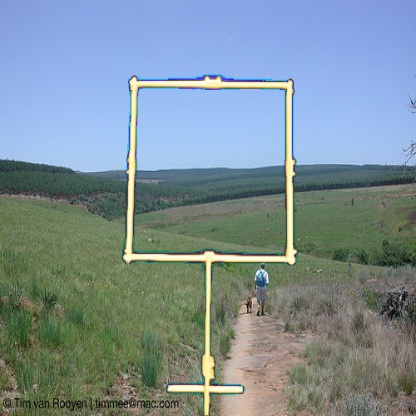
\includegraphics[width=\textwidth]{fig/voc}
	\end{minipage}
	\begin{minipage}{0.3\textwidth}
		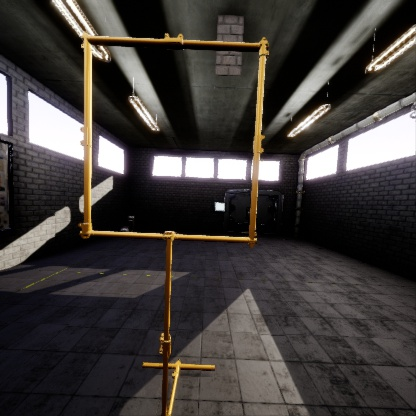
\includegraphics[width=\textwidth]{fig/sim}
	\end{minipage}
	\caption{Examples of samples with more background. On the left a sample augmented with an image from the Pascal VOC 2012 dataset. On the right a sample generated in the \textit{Daylight} Environment. Although on the left the background contains realistic data the scene does not align with the objects. Also the shadows to not fall correctly. With the simulated environment the general scene looks more realistic although the background is synthetic.}
	\label{fig:sim_vs_voc}
\end{figure}

With both methods a dataset with 20 000 samples is created. The view points are limited to frontal views.

The simulated dataset is created using \textit{Daylight} and \textit{Dark} environment which have different lightning conditions. Additionally, the backgrounds in both environments are varied such that a higher variance in background textures is achieved. Thereby the background texture that is present in the \textit{IROS} environment is not used.

For the dataset with random backgrounds 2000 view points are created in a black environment. Subsequently the black image part is replaced with a randomly selected image from the Pascal VOC dataset \todoref{voc}.

\subsection{Results}

\begin{table}
	\centering
	\input{tables/sim_vs_voc.txt}
	\caption{Performance of \textit{SmallYoloV3} in the \textit{IROS} environment when adding more variance in the background. It can be seen how including more backgrounds improves the results especially when the environment is fully simulated. Furthermore, the detector has learned to be more invariant structures that are present inside the image.}
	\label{tab:sim_vs_voc}
\end{table}

\Cref{tab:sim_vs_voc} shows the results. Selecting the backgrounds randomly thereby only led to a minor improvement. In contrast, simulating more environments and backgrounds improved the performance by 50\%.

For both methods the detectors became less subjective to patterns present in the empty part. The detector trained on simulated images achieves equal performance when there is a \textit{Cat} structure present. Also, the performance drop for the \textit{Sign} structure is less severe. Interestingly, the detector trained with random backgrounds even detects more gates when there is a \textit{Sign} structure present in the empty part.

Another observation is the higher variance in the results. Especially, when trained with random backgrounds the standard deviation is quite high. \todo{double check this with another iteration}


\subsection{Discussion}

Providing more samples from different environments was crucial for better performance. The results are even better than the ones achieved when the detector was trained and tested in the \textit{Dark} environment (\Cref{tab:all_basement}). By supplying more backgrounds the detector could learn an overall better representation. However, it seems similarly crucial to provide realistic environments. The detector trained on random backgrounds only achieved minor improvement.

Providing more variation in background also helped the detector to ignore the background. The performance drop when placing patterns inside the object is smaller.

\subsection{Conclusion}

In this section we investigated how to make the detector more invariant against changes in background and the environment. By increasing the training set with samples in front of different backgrounds this was achieved. This method even improved the results beyond its previous highest score. Thereby it seems important to provide a realistic alignment of object and scene. When simply pasting the object on random images only minor improvements could be achieved.

\section{Transferring the detector to an \ac{MAV} race}

Until now the conducted experiments where limited to relatively simple environments. In a real world application such as an \acp{MAV} race, much more objects are in sight. These can not only appear frontally but also in more difficult view angle. Furthermore, the objects can appear behind each other, such that in the empty part, another object is visible. This section studies whether the results obtained so far also apply in a more challenging environment. Therefore different architectures and training methods are evaluated on the synthetic test set described in \Cref{sec:datasets}.

Due to the challenges in this dataset we hypothesize that the detector trained so far will perform poorly on this dataset. In order to handle overlapping objects in difficult angles, such situations should be included in the training set. Yet, the amount of possible views/overlaps is large and manually constructing such examples is cumbersome especially considering the amount of samples required to train a \acp{CNN}. A simpler way is creating a scene with several objects and placing the camera randomly (within some margin) in order to cover a large variation of views on the scene. With this \textit{Random Placement} the detector can learn a general object representation and detect unseen objects from different view points. However, \acp{CNN} cannot inherently handle object rotations and variations in scale. Including too many view angles in the training set could also confuse the detector. For example from a 90° angle the investigated object appears as a straight line and is hardly detectable even for a human. If too many view angles confuse the detector the samples should be created by only using a limited set of view points.

The question remains how to choose those view points. In the application of this work the \ac{MAV} follows a predefined trajectory which is based on the a priori known race court. It needs the detections to correct its positions but the rough object position is known in advance.
Hence, the \ac{MAV} can point the camera in such a way that the object is roughly faced frontally. Subsequently, it adapts its position to fly through the gate. This behaviour can be mimicked when creating the samples. Although such a \textit{Simulated Flight} requires to create a race court an a corresponding trajectory the obtained samples should better resemble what the detector can expect in the real world.

We investigate the creation of samples with the two methods \textit{Random Placement} and \textit{Simulated Flight}. For \textit{Random Placement} 600 samples are created by heuristically choosing the following distributions:

\begin{equation}
x = \mathcal{U}(-30,30),\quad y = \mathcal{U}(-20,20),\quad z = \mathcal{N}(-4.5,0.5)),\quad
\phi = \mathcal{U}(0,0.1\pi),\quad \theta = \mathcal{U}(0,0.1\pi),\quad \psi = \mathcal{U}(-\pi,\pi)
\label{eq:distroexp}
\end{equation}
Where $\mathcal{U}(a,b)$ is a uniform distribution with borders $a$ and $b$; $\mathcal{N}(\mu,\sigma)$ a Gaussian distribution with mean $\mu$ and variance $\sigma$. The labels are compared to the ones from the synthetic dataset described in \Cref{sec:datasets}.

For \textit{Simulated Flight} the dynamic model of a quadcopter is used. Several race courts are created and the camera follows a predefined trajectory through these race courts.

\begin{figure}
	\begin{minipage}{\textwidth}
		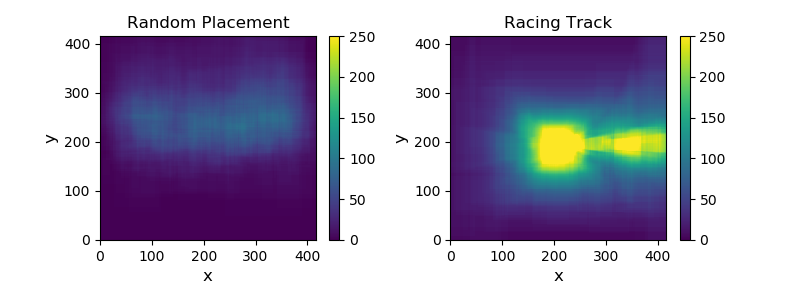
\includegraphics[width=\textwidth]{fig/heatmap_camplace}
		\caption{Object appearances in 2D when generating 600 samples with \textit{Random Placement} and  \textit{Simulated Flight}. Each pixel value corresponds to the number of labels that cover this particular pixel. In the simulated flight objects appear mostly centred on the horizontal line.}
		\label{fig:heatmap_camplace}
	\end{minipage}
	\begin{minipage}{\textwidth}
	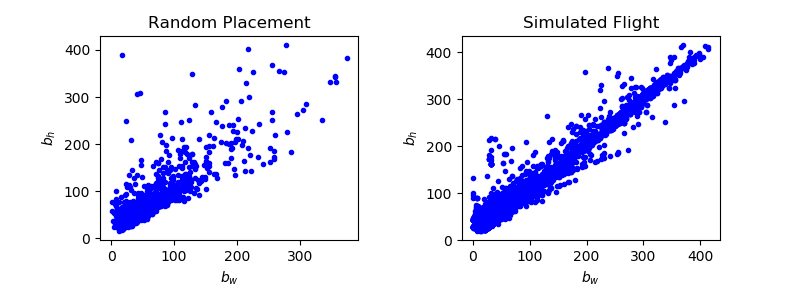
\includegraphics[width=\textwidth]{fig/ar_train}
	\caption{$b_h$ and $b_w$ of 600 samples created with \textit{Random Placement} and  \textit{Simulated Flight}. When the object is faced frontally the aspect ratio is 1.1/1. It can be seen how with \textit{Simulated Flight} much more close up samples are created. On the other hand \textit{Random Placement} covers a broader range of view angles.}
	\label{fig:aspect_ratio_camplace}
	\end{minipage}
\end{figure}

\Cref{fig:heatmap_camplace} shows the label distribution when created with the two methods. Thereby each pixel value corresponds to the number of labels that cover this particular pixel. It can be seen how, when following the race track most of the objects are centred and distributed across the horizon, as camera focuses the next object frontally most of the time. In contrast,\textit{Random Placement} leads to more evenly distributed object locations. 

\Cref{fig:aspect_ratio_camplace} shows $b_h$ and $b_w$ of 600 samples created with the two methods. Although the actual view angle can not be inferred from these dimension, the plot gives an idea on how the labels look like. When the object is faced frontally the aspect ratio is 1.1/1. It can be seen  \textit{Random Placement} covers a broader range of view angles but does not create many samples with large objects. The reason is that the field of view gets smaller as objects get closer. Hence, the camera ending up exactly in front of the object is relatively low. On the other hand with \textit{Simulated Flight} does not cover many view points where $b_h >> b_w$. In the created race courts these view angles do not seem to be present.

We investigate to what extent the detector can generalize across view points. We hypothesize that a detector trained with \textit{Simulated Flight} performs better in a simulated \ac{MAV} race than a detector trained with \textit{Random Placement}. 

Training sets with 20 000 samples each are created using \textit{Random Placement} and \textit{Simulated Flight}. The scenes are created with the environments introduced in \Cref{sec:environments}. Additionally, the background textures are varied during data generation. For \textit{Random Placement} the gates are placed throughout the room, subsequently the camera is placed according to \Cref{eq:distroexp}. For \textit{Simulated Flight} 3 race courts with corresponding trajectories are created. It should be noted that the race court present in the test set is not part in either of the training sets. 

During data generation it can happen that the camera ends up at a view point where the object is only visible as a dot or a straight line. Including such samples in the training confused the detector in initial experiments. Therefore, we set a limit to aspect ratio and bounding box size. For \textit{RandomPlacement} samples outside that limit are excluded, for \textit{SimulatedFlight} only the labels are removed. The aspect ratio is limited to a minimum  of $\frac{1}{3}$ a maximum of 3.0. For the object size a minimum of 1 \% of the image size is chosen.


\subsection{Results}

The results are presented in \Cref{fig:view_size}. Predicted and true labels are assigned to bins based on their covered area $A_O=b_w*b_h$. Subsequently $ap_{60}$ is evaluated for each bin. 
\begin{figure}[hbtp]
	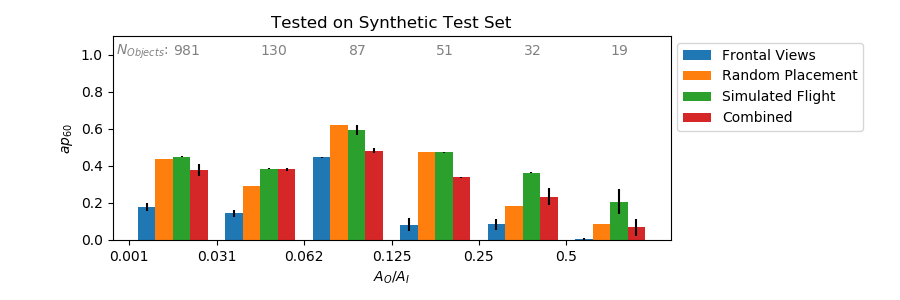
\includegraphics[width=\textwidth]{fig/view_size}
	\caption{Results of different methods to include more samples in the training set. The results are clustered based on the size of the true/predicted bounding box. It can be seen how the network that contained only frontal views performs poorly when applied in the simulated \ac{MAV} race track. The network trained with images obtained with \textit{Simulated Flight} outperforms the network trained on samples obtained with \textit{Random Placement} for larger object sizes.}
	\label{fig:view_size}
\end{figure}

\begin{figure}[hbtp]
	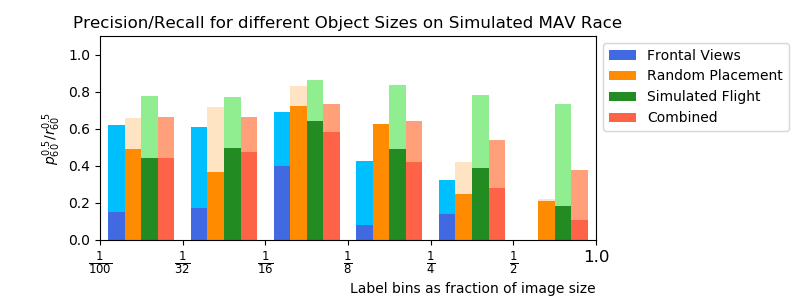
\includegraphics[width=\textwidth]{fig/view_precision_recall}
	\caption{Precision and Recall at a confidence level of 0.5 of different methods to generate data. The results are clustered based on the size of the true/predicted bounding box. For each method and each bin precision and recall are shown. Precision is the lighter coloured bar. It can be seen how for \textit{Simulated Flight} only the recall drops for larger objects. With \textit{Random Placement} included, the precision drops similarly.}
	\label{fig:view_size_pr}
\end{figure}

\textit{Frontal Views} is the network trained in the previous section. Its training set contained only frontal views and no overlap. It can be seen how it performs poorly when simulating a whole \ac{MAV} race. \textit{Random Placement} achieves competitive performance for smaller object sizes until 25\% of the input image. However, the performance drops below 20\% for larger objects. \textit{Simulated Flight} achieves competitive performance on all bins. Only for objects of a size between 6.2\% - 12.5\% of the input image the random placement performs slightly better. In most bins combining both methods led to worse results than each of the methods individually.

Overall a significant drop in performance can be seen compared to the test sets of the previous sections. Only on the bin for objects of a size between 6.2\% - 12.5\% of the input image the networks achieve a comparable performance of 69 \%. This bin seems to be the optimal distance for all networks. Especially for larger objects the performance decreases.

\subsection{Discussion}

In the results it can be seen how the detectors struggle in the more challenging environment of a \ac{MAV} race. Compared to the results on the simple dataset of the previous section, a drop in performance can be seen for all detectors. Including more view points in the training set helped counteracting against this drop. The networks trained with more view points perform significantly better than the network which was only trained on frontal views.

Yet including to many view points seems to confuse the detector. The network trained with \textit{Random Placement} performs poor for larger objects. Combining \textit{Random Placement} and \textit{Simulating Flight} leads overall to a deterioration in performance. In contrast, the network trained with \textit{Simulating Flight} only, achieves a higher performance. This is mainly achieved because the precision stays high. The detectors with \textit{Random Placement} produce more false positives compared to the network trained with \textit{Simulating Flight}.

\textit{Random Placement} and \textit{Simulating Flight} are limited in a way that they do not give control of which exact view points are present in the training set. A more sophisticated method could be the controlled creation of particular view points. This way a certain distribution of scales and angles could be created. On the other hand this creates other questions such as in what way to include overlap etc. Furthermore, enough variation in background would be required for each view point. Controlling each of these parameters manually would require a lot of engineering work or a further extension of the created data generation tool. Nevertheless, it would be worth investigating and could be addressed in future work.

Overall a performance drop for larger objects can be seen. This is somewhat surprising as the object should be better visible when it is larger. However, the closer the camera gets, the less context is visible and the more likely it is that a part of the object is out view. This could be the reason for the drop in performance for larger objects. An experiment that would show whether this is true could be done by training the network without the pole and testing the model again.

\subsection{Conclusion}

In this section we evaluated how the detector performs when applied in a simulated \ac{MAV} race. We hypothesized that the performance will decrease as more view points and overlapping angles are visible. The results confirm this hypothesis.

Furthermore, we investigated whether the detector can learn to detect the object from many view points. Although this seems possible, it comes at cost of precision for larger object sizes. We can conclude that restricting the network to a subset of view points is crucial to keep a better performance for larger objects.



\section{Optimizing the Architecture}
\label{sec:exp_arch}
The baseline network architecture is optimized to detect solid feature rich objects of multiple classes. In order to sufficiently represent and distinguish such complex objects many weights are required. This leads to a high computational complexity and longer inference time. Also, more weights require typically more data to train and are more prune to overfit to a training set. The features of \acp{EWFO} are relatively simple hence less weights should be required. This section investigates whether equal performance can be reached when using a more shallow/thinner architecture.

The width in a \acp{CNN} determines how many features can be extracted in one layer. Wider networks can extract and retain more information than thinner layers. As the information in \acp{EWFO} is limited to basic geometric shapes and colour, we hypothesize a thinner network should be able to learn the detection task equally well. Only when reducing the width too strong the performance should drop significantly as a minimum of weights is required. We examine this by reducing the number training networks with a thinner architecture. Therefore the number of filters in each layer of the \textit{SmallYoloV3} network are reduced to $\frac{1}{2}$, $\frac{1}{4}$, $\frac{1}{8}$ and $\frac{1}{16}$ of its original number. The network is trained on the training set consisting of various racing courts. All architectures are tested on the simulated \ac{MAV} race introduced in \Cref{sec:datasets}.

The depth of a network has multiple effects. Deeper networks contain more non-linear elements and can thus represent more complex functions/features. \acp{EWFO} have simple features and thus only a few layers should be required. In fact the features that are relevant to detect an \acp{EWFO} are typically lines on the border of its location. Hence, a detector would only need to detect those edges in order to determine whether an object is present. This should be possible with a few amount of layers. On the other hand in a \acp{MAV} race the objects appear overlapping and in difficult angles. In such cases the above is not valid anymore. For overlapping objects a detector would need to distinguish which line/edge belongs to which object. Such complex relations can be better represented with a deeper network. We investigate these hypotheses in an experiment. Therefore we remove layers but use larger pooling operations. The network is trained on the training set consisting of various racing courts introduced in the previous section. Additionally, \textit{VGGYoloV3} is trained on the data. All architectures are tested on the simulated \ac{MAV} race introduced in \Cref{sec:datasets}.

It should be noted that throughout the thesis many more architectures have been evaluated. For example using larger kernels, dilated convolutions, varying pooling operations at different layers. However, in the end none of these architectures led consistently to an increased efficiency (performance/weights). While under certain conditions improvements could be observed, these usually disappeared when applying the detector on a different test set. Overall reduction in weights led to a similar decrease in performance as can be seen in the results of this experiment. Therefore, we keep the basic structure of the baseline architecture as it follows a pattern that is intuitive to understand. We show how the results change when varying the parameters of the architecture on a high level basis (depth/width).

\section{Results}

\Cref{tab:depth} shows the results of networks with varying depth. The best network on simulated \ac{MAV} race has 9 layers. Further increasing depth does not lead to an improvement in performance. In contrast reducing the number of layers decreases the performance gradually. 

\begin{table}[hbtp]
	\centering
	\input{tables/depth.txt}
	\caption{Performance of networks with varying depth on the simulated \ac{MAV} race. It can be seen how on the more complex test set depth only improves the performance until 9 layers.}
	\label{tab:depth}
\end{table}

\Cref{tab:width} shows the results of networks with varying width. The best architecture is the baseline with 51\%. Reducing to the width leads to a decrease in performance, particularly when only half the amount of filters is used. A further reduction in weights leads to a more gradual decrease in performance in steps of 1-2\%. The lowest result is obtained when using a width of $\frac{1}{16}$.

\begin{table}[hbtp]
	\centering
	\input{tables/width.txt}
	\caption{Performance of networks with varying depth on the simulated \ac{MAV} race. }
	\label{tab:width}
\end{table}

\subsection{Discussion}

Similarly to the results in \Cref{sec:empty} the very deep network does not improve in performance. Hence, depth does not seem to help when detecting objects with more overlap and in difficult view angles. However, a certain amount of layers seems to be crucial. When decreasing the number of layers further than 9 the performance gradually decreases. A possible reason is that with less layers the pooling has to be increased in order to keep the receptive field large enough. Yet aggressive pooling removes spatial information quickly. While this is of less influence for the detection task, it can be harmful for the localization. 

For lower width we hypothesized that the performance will only be effected for a very small amount of filters. However, the results show how the performance decreases already with half the amount of filters by 8\%. Further reduction leads to smaller decreases until a performance of 38\% is reached. That is despite using only 0.4\% of the weights of the original architecture the performance drops only by 13\%. 


\subsection{Conclusion}

We investigated how depth affects the detection performance. Our hypothesis was that a deeper network could perform better at detecting objects in difficult angles or higher overlap. However, we could not confirm this hypothesis. Yet decreasing the depth to less than 9 layers also hurts the performance. It seems that too aggressive pooling is bad for the object localization.

We investigated how width affects the performance for the detection of \acp{EWFO}. We hypothesized that due to the low variance in the investigated object and the simple features, less filters are required than in the baseline architecture. We can not really confirm or reject this hypothesis. Although a performance drop can be observed it is relatively low compared to the amount of weights that are removed.


\section{Transferring the detector to the real world}

After having gained several insights in simulation it is time to perform experiments on real data. This section investigates the reality gap and several methods to reduce it.

As a test set the real world dataset introduced in \Cref{sec:datasets} is used. The examples in \Cref{fig:example_real_set} show several properties that are different to the samples created in simulation. The objects used in this dataset consist of square bars and a black pole. In contrast the \ac{CAD} models used for synthesizing data consist of round bars and are uniformly coloured. Also, the aspect ratio between both objects is different. In contrast to the synthetic objects, the objects in the real world set are more wide than high. Finally, the colour is not exactly the same. A network only trained on the available \ac{CAD} models is likely to overfit to the colour and object shape. In order to evaluate this hypothesis a new 3D Model is created and samples are included in the training set. The new model can be seen in \Cref{fig:mavlabgateexample}.

\begin{figure}[hbtp]
	\centering
	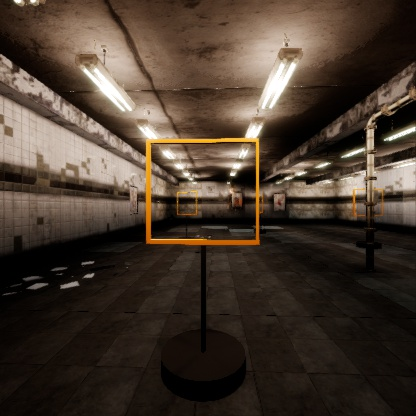
\includegraphics[width=0.3\textwidth]{fig/mavlabexample}
	\caption{In order to increase the variance in object appearance a new 3D-Model is created using \textit{AirSim}. It contains a black pole and square bars.}
	\label{fig:mavlabgateexample}
\end{figure}

Furthermore, it can be seen how motion blur and lens distortion change object appearance. We hypothesize that including such effects in the training data can improve the performance on the real data. The experiments in \cite{Carlson2018} show how the incorporation of sensor effects particularly improves the performance of models learned on fully synthesized data. We study this incorporation by applying image augmentation with the models introduced in \Cref{sec:postprocessing}.

The detector is trained with 20 000 samples where 3000 are generated with the new 3D model. During training one or several image augmentation methods. The parameters chosen visually:

\begin{itemize}
	\item Distortion: $k_1 = k_2 = 0.7$.
	\item Blur: $\sigma$ is drawn from a uniform distribution: $\mathcal{U}(0.1,1.5)$.
	\item Chromatic: $t^R_x$,$t^R_y$,$s^G$,$t^B_x$,$t^B_y$ are drawn from $\mathcal{U}^R(-2,2)$, $\mathcal{U}^G(0.99,1.01)$,$\mathcal{U}^B(-2,2)$.
	\item $\Delta H$,$\Delta S$,$\Delta V$ are drawn from $\mathcal{U}^H(.9, 1.1)$, $\mathcal{U}^S(0.8, 1.2)$, $\mathcal{U}^V(0.8, 1.2)$
\end{itemize}

Initial experiments show relatively poor results on the \textit{Hallway} dataset. In this data set the objects are placed in front of a window which causes the objects to appear quite dark. Also the background is light and contains many details. We hypothesize that the lack of colour and the background confuse the detector. In order to examine two additional networks are trained:

\begin{itemize}
	\item \textit{Grey} is trained by transforming 50\% of the images to grayscale images during training. This should force the network to learn more colour invariant features and thus improve the results on the \textit{Hallway} dataset. 
	\item \textit{VOC Background} is trained by including the images created with backgrounds chosen from the VOC dataset (\Cref{sec:exp_background}. We hypothesize that by providing more variance in the background, the network will be more robust against details in the background. This should improve the results on the \textit{Hallway} dataset.
\end{itemize}

Next to evaluating the network on real data a comparison to the baseline is given. \textit{SnakeGate} is evaluated on each of the test sets. The colour filter is tuned for each environment. As the initial sampling of \textit{SnakeGate} is stochastic, mean and standard deviation of 5 repeated runs are presented.

\subsection{Results}

\begin{figure}[hbtp]
	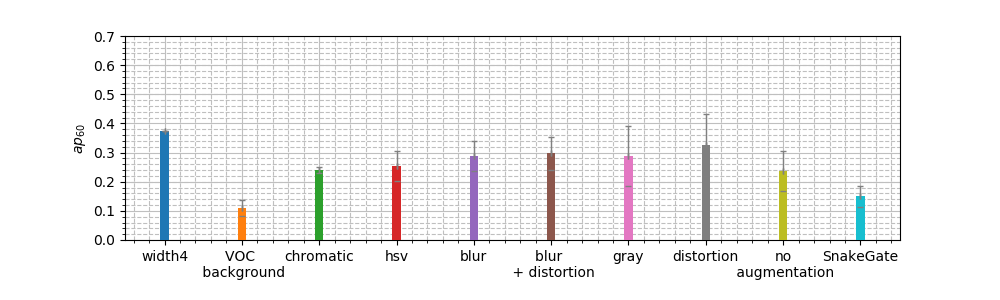
\includegraphics[width=\textwidth]{fig/augmentation_overview}
	\caption{An overview over all applied augmentation methods. The results are presented as the mean $ap_{60}$ over the three data sets. The results of 4 runs are reported. It can be seen how \textit{blur} and \textit{distortion} as well as \textit{grey} lead to an improvement in performance compared to not using augmentation.}
	\label{fig:augmentation_overview}
\end{figure}

\Cref{fig:augmentation_overview} shows the mean performance of networks trained with different augmentation methods. Variations in \ac{HSV}, chromatic aberration as well as including backgrounds from the Pascal VOC datasets lead to a deterioration in performance compared to not using any augmentation. In contrast, including blur, distortion and gray images leads to an improvement. The overall best results can be achieved by including distortion and gray images in the training.

\begin{figure}[hbtp]
	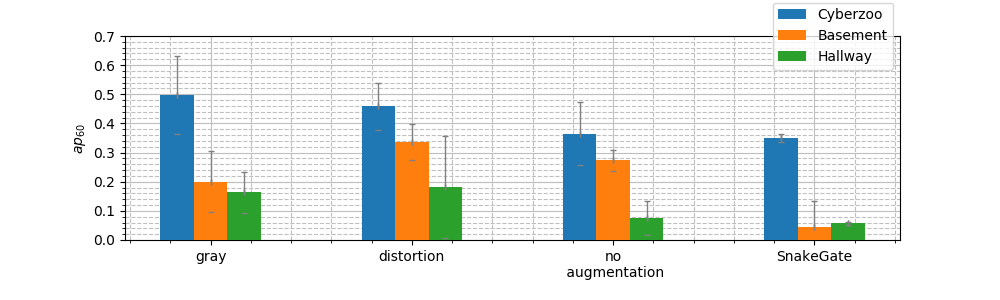
\includegraphics[width=\textwidth]{fig/augmentation}
	\caption{The results of \Cref{fig:augmentation_overview} in more detail for the different data sets. It can be seen how \textit{grey} improves the performance mainly on \textit{Cyberzoo} and \textit{Hallway} while the performance on \textit{Basement} gets worse. In contrast \textit{distortion} leads to a more overall improvement. Particularly for \textit{Cyberzoo} and \textit{Hallway} the variance in the results is high.}
	\label{fig:augmentation}
\end{figure}

\Cref{fig:augmentation} shows the results for the best augmentation methods in more detail. It can be seen how \textit{grey} improves the performance mainly on \textit{Cyberzoo} and \textit{Hallway}. In contrast, on \textit{Basement} the performance drops compared to not using any augmentation. \textit{Distortion} leads to a more even improvement for all data sets.

Particularly for \textit{Cyberzoo} and \textit{Hallway} the variance in the results is high.

\Cref{fig:example_cyberzoo,fig:example_basement,fig:example_hallway} show example predictions on the various data sets of the network trained with distortion. On \textit{Cyberzoo} and \textit{Basement} several very accurate predictions can be seen, even under heavy occlusion. On \textit{Hallway} this is rather an exception. Yet on all data sets several images where the object is clearly visible, are wrongly or not at all detected.

\begin{figure}[hbtp]
\centering
\begin{minipage}{0.24\textwidth}
	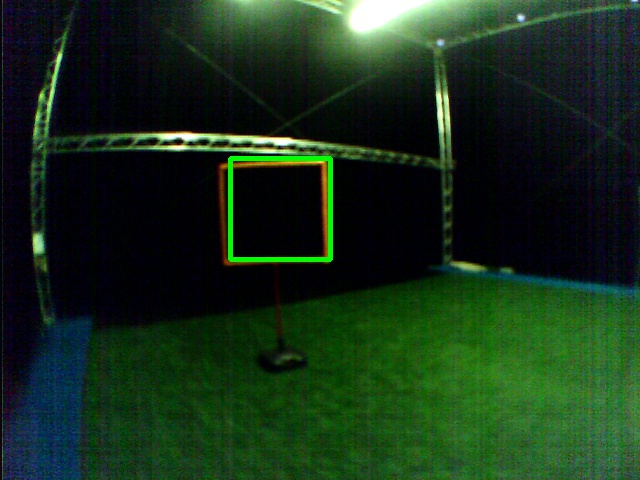
\includegraphics[width=\textwidth]{fig/examples/cyberzoo_nice1.jpg}
\end{minipage}
\begin{minipage}{0.24\textwidth}
	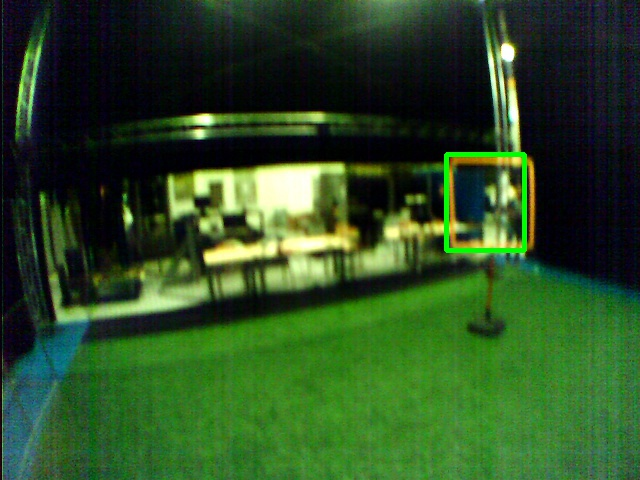
\includegraphics[width=\textwidth]{fig/examples/cyberzoo_nice2.jpg}
\end{minipage}
\begin{minipage}{0.24\textwidth}
	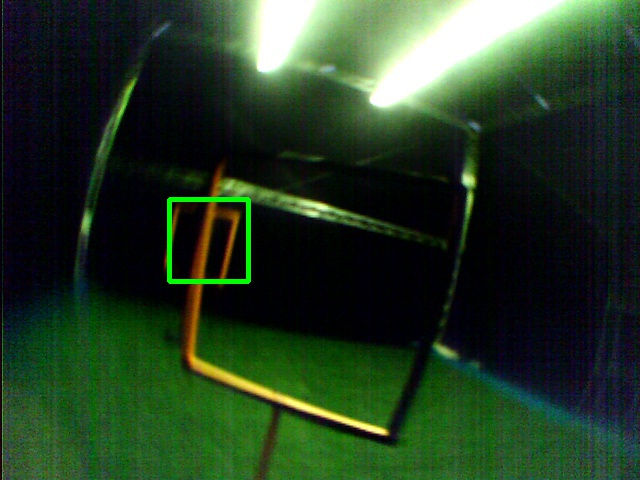
\includegraphics[width=\textwidth]{fig/examples/cyberzoo_notnice1.jpg}
\end{minipage}
\begin{minipage}{0.24\textwidth}
	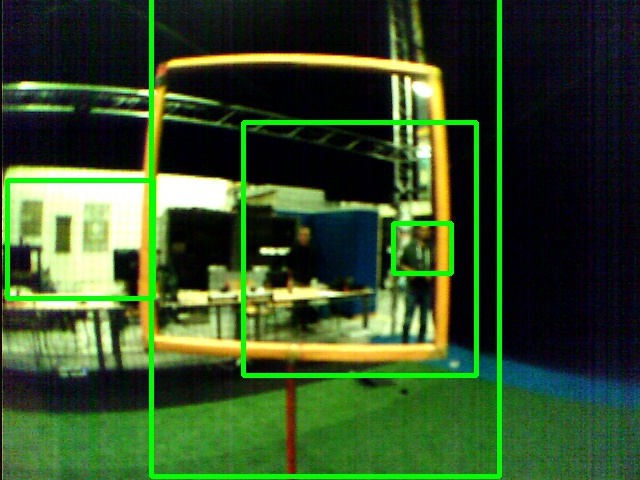
\includegraphics[width=\textwidth]{fig/examples/cyberzoo_notnice2.jpg}
\end{minipage}
\caption{Predictions in the \textit{Cyberzoo} environment of the network trained with distortion. Several gates are detected with good localization, even when occluded by another gate (3.). Yet the gate which is in front is not detected. Also, the perfect visible gate (4.) is not well detected. Instead many false positives are predicted.}
\label{fig:example_cyberzoo}
\begin{minipage}{0.24\textwidth}
	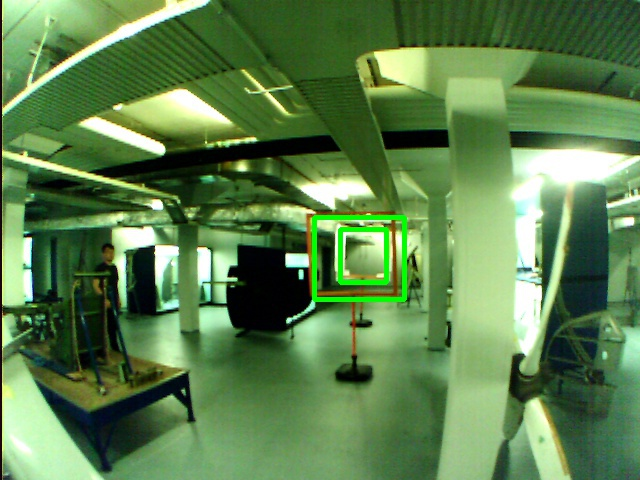
\includegraphics[width=\textwidth]{fig/examples/basement_nice1.jpg}
\end{minipage}
\begin{minipage}{0.24\textwidth}
	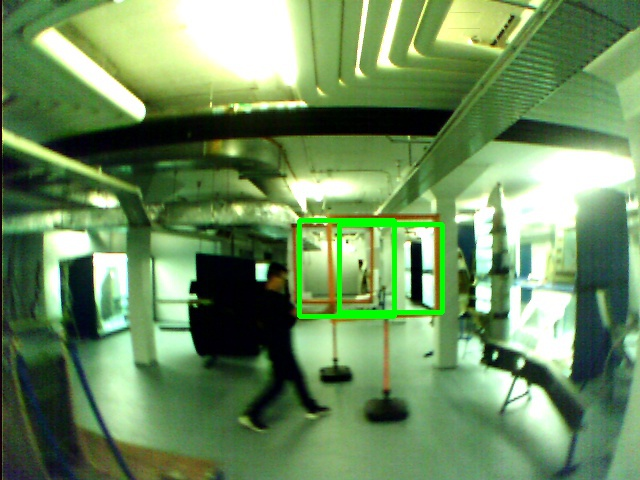
\includegraphics[width=\textwidth]{fig/examples/basement_nice2.jpg}
\end{minipage}
\begin{minipage}{0.24\textwidth}
	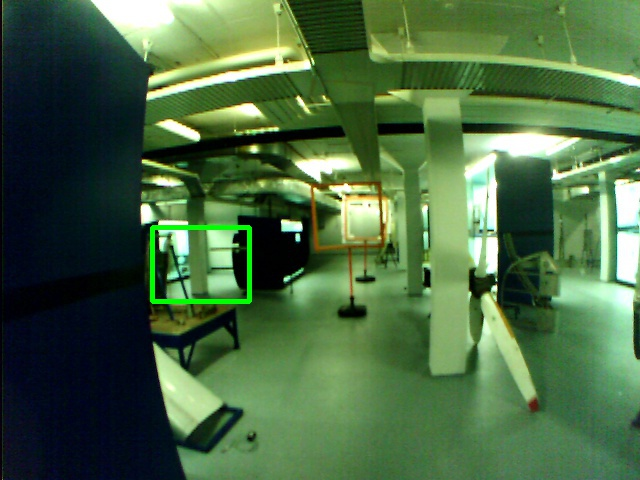
\includegraphics[width=\textwidth]{fig/examples/basement_notnice1.jpg}
\end{minipage}
\begin{minipage}{0.24\textwidth}
	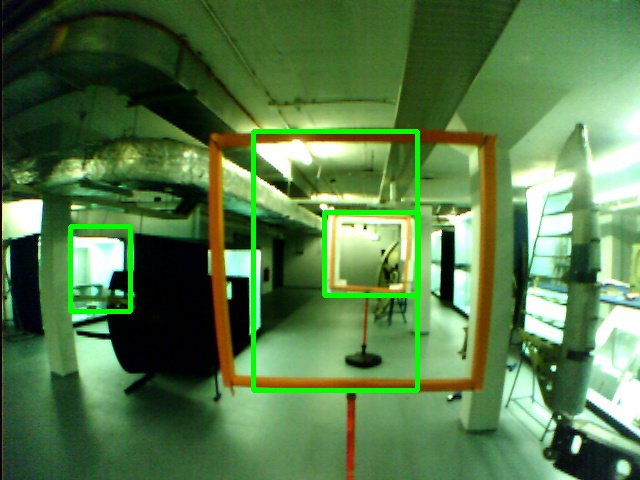
\includegraphics[width=\textwidth]{fig/examples/basement_notnice2.jpg}
\end{minipage}
\caption{Predictions in the \textit{Basement} environment of the network trained with distortio. The network produces very nice detections in cases of heavy occlusion (1 and 2). However, in other cases where the gate is visible at least equally well (3 and 4) the gate is not detected or with bad localization.}
\label{fig:example_basement}
\begin{minipage}{0.24\textwidth}
	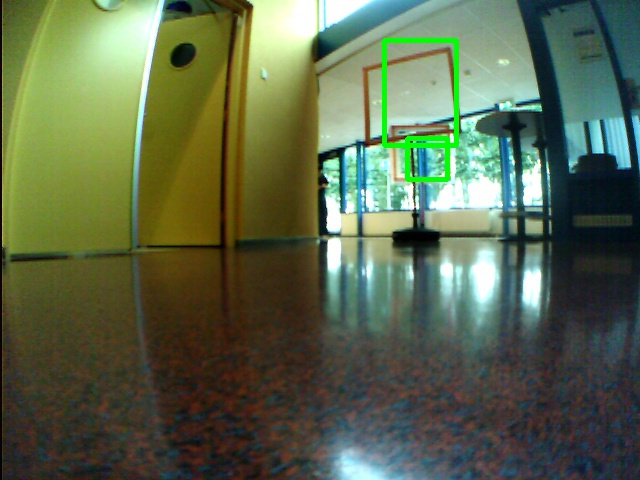
\includegraphics[width=\textwidth]{fig/examples/hallway_nice1.jpg}
\end{minipage}
\begin{minipage}{0.24\textwidth}
	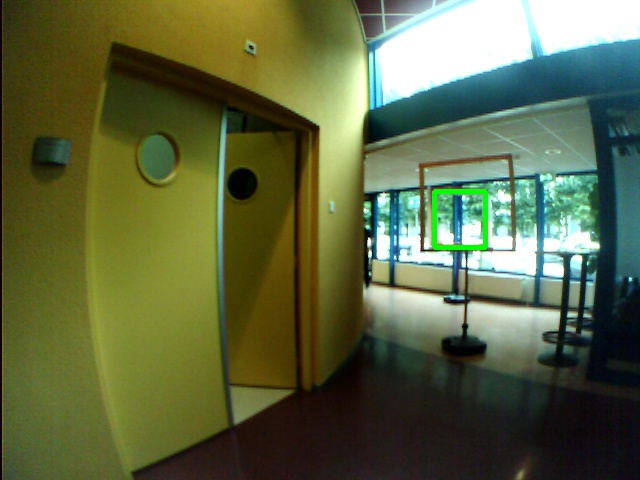
\includegraphics[width=\textwidth]{fig/examples/hallway_nice2.jpg}
\end{minipage}
\begin{minipage}{0.24\textwidth}
	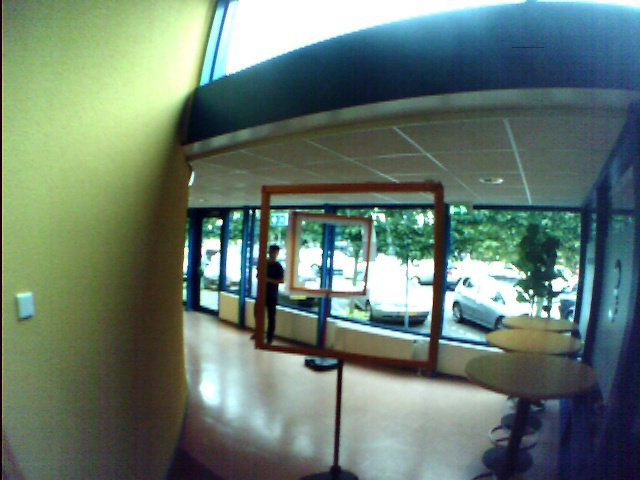
\includegraphics[width=\textwidth]{fig/examples/hallway_notnice1.jpg}
\end{minipage}
\begin{minipage}{0.24\textwidth}
	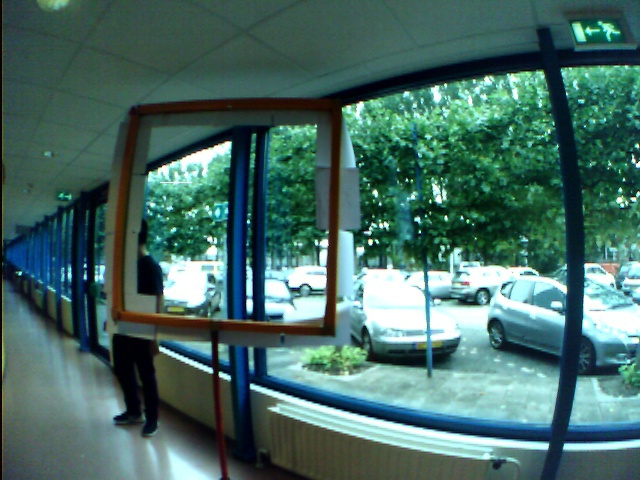
\includegraphics[width=\textwidth]{fig/examples/hallway_notnice2.jpg}
\end{minipage}
\caption{Predictions in the \textit{Hallway} environment of the network trained with distortion. In some images (1 and 2) the network predicts a half way correct bounding box. Yet in the majority of images such as 3 and 4 the gate is not detected, although clearly visible. }
\label{fig:example_hallway}
\end{figure}

\subsection{Discussion}

In this experiment the detector is evaluated on real data. Compared to simulation, only on \textit{Cyberzoo} comparable results can be achieved. On the more difficult data sets \textit{Hallway} and \textit{Basement} the performance drop is quite significant. On \textit{Hallway} almost no detection can be achieved. Hence, there seems to still be a big reality gap.

Where exactly the gap lays in is difficult to identify. Among image augmentation that addresses the colour feature such as \textit{HSV} and \textit{Grey} only \textit{Grey} leads to an improvement. Thereby the main improvement is obtained on the \textit{Cyberzoo} dataset where illumination/colour is of smaller influence. 

Lens distortion and blurring leads to an overall improvement on the datasets. However, the improvement cannot be particularly appointed to certain samples that suffer from heavy distortion or motion blur. Also, a high variance in the results can be observed which makes it difficult to conclude something. This holds especially for \textit{Basement} and \textit{Hallway} which are comparable small data sets. Potentially a more sophisticated real world test set could give better insights.

For \textit{Hallway} the results are particularly low. We hypothesized that the reason is the noise in the background and that including backgrounds from the Pascal VOC dataset can lead to an improvement on this dataset. However, including these samples seem to further confused the detector. The results deteriorate. On \textit{Hallway} the images are also taken against light background which makes the gate appear dark. We hypothesized that including grey images in the training improves the results on this dataset. We can observe an improvement from 8\% to 16\% by applying this technique. Hence, it seems that the technique helped a bit however it is not the predominant problem on this dataset.

Compared to \textit{SnakeGate} the network achieves better results. Especially, when including distortion the results improve by 10\%. Hence, the learning based detector seems to have learned a more robust detection of the racing gates.

In several examples in \Cref{fig:example_cyberzoo,fig:example_basement,fig:example_hallway} it can be seen how clearly visible objects are not detected. In simulation this is less of a problem. Hence, it seems that there is still a gap between the simulated data and the one present in the real world.

\subsection{Conclusion}

We investigated how the detector performs in the real world and if image augmentation can bridge the reality gap. We can conclude that image augmentation can improve the results on the real world data. In particular the modelling of lens distortion and the incorporation of grey images improve the results. Nevertheless, these results are preliminary as the variance in the results does not allow a final conclusion. Potentially, a more sophisticated test set could give more insights.

In more difficult environments the performance drops significantly. Also, several clearly visible objects can not be detected. As this typically not happens in simulation we can conclude that there is still a large reality gap. Potentially, the results can be improved when including real world data in the training set. Such experiments should be conducted in future work.

Overall an improvement of the learning based detector compared to the baseline can be reported. The results in simulation show potential further improvement with better training data.


\section{Deploying the detector on a \ac{MAV}}
\}
In the application of the detection of \acp{EWFO} on a \acp{MAV} detection accuracy is only one important metric. Equally relevant are inference speed and energy requirements. The example control loop in which the detector of this work is integrated, contains a filtering stage which fuses measurements of different sensors over time to infer a global state. This stage can deal with outliers and henceforth it can be more important to have more bad detections in high frequency than only slow but good ones. This section studies the deployment of a detector for \acp{EWFO} on a \ac{MAV} in the example of the target system of this work. Therefore the performance-accuracy trade-off is studied and an experiment in a real world flight is conducted.

As explained in \Cref{sec:background} the execution time strongly depends on the used hardware as well as its low level implementation. Therefore the inference time of several layers is measured on the JeVois using the \textit{Darknet} framework. The results are displayed in \Cref{fig:bottleneck_jevois}. Each sample corresponds to the number of computations and their computational time in one layer. Dashed lines connect samples at the same resolution. It is apparent how the same amount of computations at a spatial resolution of 20x15 is more than 4 times faster than at a resolution of 160x120. We assume this is because parallelism is better exploited at the lower scale.

\begin{figure}[hbtp]
	\centering
	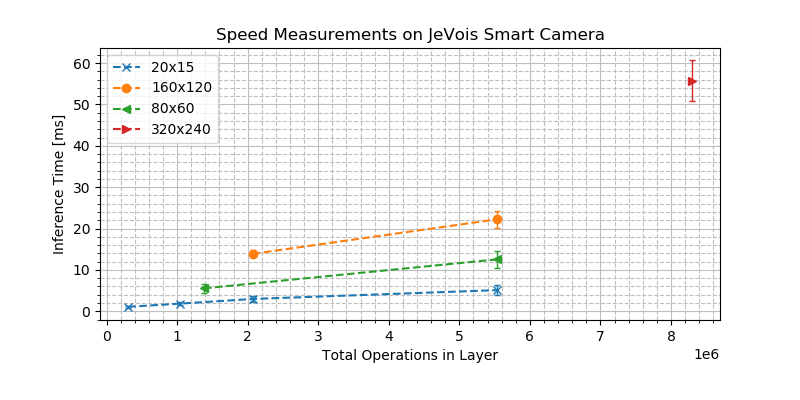
\includegraphics[width=0.8\textwidth]{fig/bottleneck_jevois}
	\caption{Inference Time of different layers on the JeVois. Each sample corresponds to the inference in a single layer. Dashed lines connect samples at the same resolution. It can be seen how an operation at a higher spatial resolution is significantly slower.}
	\label{fig:bottleneck_jevois}
\end{figure}

This means most speed can be gained when reducing the number of computations in the early layers where the spatial resolution is high. In \Cref{sec:exp_arch} it could be seen that already a small amount of filters in the early layers is enough to detect \acp{EWFO}. However, even evaluating 4 kernels at a resolution of 320x240 already takes 55 ms (\Cref{fig:bottleneck_jevois} red triangle). A total network of that size would require more than 100 ms and is thus too slow to be deployed in the control loop.

Current research mostly addresses to reduce the computations when the convolved volumes are deep or the operations are performed on \acp{CPU} that do not support floating point operations. However, the bottleneck on the JeVois happens at shallow volumes and the hardware can perform floating point operations. Furthermore, \acp{EWFO} consist of thin elements that are spread over large parts of the image. Hence, we hypothesize that simply reducing the image resolution will lead to large drops in performance. An alternative is to increase the stride parameter in the early layers of the network. This reduces the number of locations at which the kernel is evaluated. \acp{EWFO} are sparse and spread over large parts of the image, while most of the image does not contain useful information. Hence, we hypothesize that increasing the stride parameter in the early layers will perform better than reducing the image resolution.

In order to evaluate our hypotheses the network is trained with different architectures. Subsequently, performance on the real data and inference time on the \textit{JeVois} are measured.

The \textit{JeVois} supports aspect ratios of 4:3 and resolutions of 160x120, 320x240 and 640x480. Although, the detector does not depend on the image size, the object appearance can change at lower image resolution. Hence, during training the images are scaled to 160x160 or 320x320 respectively. The anchor boxes are scaled in similar fashion. Finally, as the input image resolution decreases, the output grid size decreases by the same factor. This is not desirable as the output resolution should stay the same. Hence, when decreasing the input image pooling layers are removed such that the output grid stays at 20,20 or 10,10 respectively.

\section{Results}

\Cref{fig:ap_speed_tradeoff} shows the results of the conducted experiments. Next to the different architectures time and performance of \textit{SnakeGate} are given. \textit{SnakeGate} has high variance in time as its execution time depends on the colour filter stage. If no object is visible and everything is filtered by the colour filter  \textit{SnakeGate} has an execution time of less than 1ms. For detections however some minimum execution time is required.

The plot shows how the different networks are generally slower than \textit{SnakeGate}. Only the network applied at 160x120 gets with 55 ms/frame near the maximum execution time of \textit{SnakeGate}. In terms of average precision the networks show a better performance. The best results of 32\% can be obtained by the network with one stride layer. Replacing more pooling layers with larger strides leads to a drop in performance but an increase of inference speed.

\begin{figure}[hbtp]
	\centering
	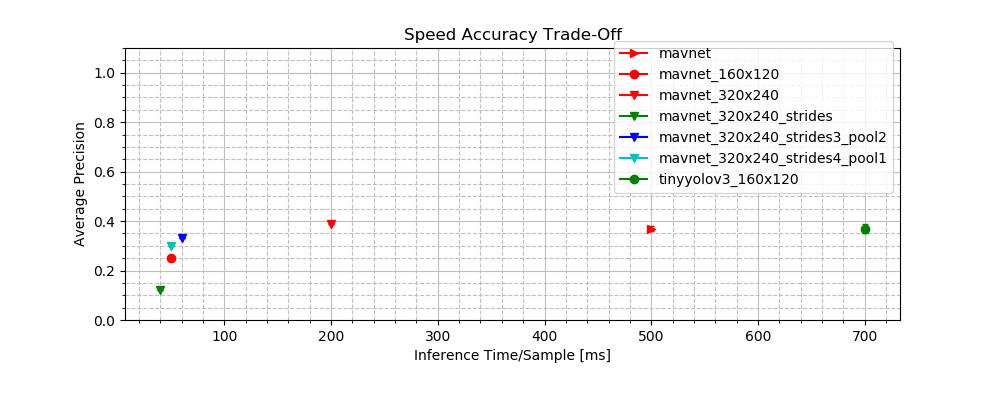
\includegraphics[width=0.8\textwidth]{fig/ap_speed_tradeoff}
	\caption{Inference Time of different layers on the JeVois. Each sample corresponds to a single layer. On the x-axis the total number of multiplications in that layer is displayed. It can be seen how an operation at a higher spatial resolution is significantly slower.}
	\label{fig:ap_speed_tradeoff}
\end{figure}


\subsection{Discussion}

In this section different methods to increase the speed of the detector were investigated. As expected the performance is better when keeping a higher resolution but increasing the stride parameter. At a resolution of $160\times120$ the performance of the detector drops almost to the level of \textit{SnakeGate}. In contrast the network with one stride layer achieves the best results.

Replacing the first pooling layers with larger strides gives a speed up of 17 ms/frame without loosing any performance. Further replacing the pooling layers leads a stepwise decrease in performance. Hence, replacing the pooling layers with larger strides can be used to trade-off between performance and inference speed.

\subsection{Conclusion}

In this experiment we evaluated the trade-off in terms of speed and accuracy on the \textit{JeVois} and compared it to the baseline. It could be seen how replacing pooling layers with larger strides can be used to trade-off inference speed and detection performance. 

Overall the same inference speed as \textit{SnakeGate} can not be achieved by the network. Hence, we can conclude that the learning based detector improves detection performance at cost of inference speed.





